\documentclass[12pt, a4paper]{article}

\usepackage[ngerman]{babel}	% Für die deutsche Sprache
\usepackage{karnaugh-map}   % Für KV-Diagramm (Doku vorhanden)
\usepackage{cite}		% Für ein Quellenverzeichnis
\usepackage{amsmath}	% Sorgt für den Mathe Modus		
\usepackage{graphicx}	% Ist für die einbindung von Bildern dar
\usepackage{tabularray}	% Fügt schöne Tabellen hinzu
\usepackage{xcolor}		% Erlaubt farben für das Dokument
\usepackage{colortbl}	% Erlaubt das einfärben von Tabellen
\usepackage{geometry}	% Ermöglicht das ändern der Seitenränder
\usepackage{hyperref}	% Macht Links möglich
\usepackage[
	skip = 0pt,		% Falls man Platz zwischen Paragraphen braucht
	indent = 0pt			% Einrückung für einen neuen Paragraphen
]{parskip}

\usepackage{enumitem}

\usepackage{subcaption}

% ----------  Einstellungen  ----------------------------------------------

\geometry{
	left = 3.15cm, % Normaler Seitenabstand Links
	right = 3.15cm, % Normaler Seitenabstand Rechts
	top = 3.56cm, % Normaler Abstand von oben
	bottom = 3.56cm % Normaler Abstand von unten
}

\hypersetup{
	colorlinks = true, % Erlaubt Farbige Links
	linkcolor = black, % Macht das Inhaltsverzeichnis Schwarz
	urlcolor = blue,   % Macht eingebundene URLs Blau
	citecolor = red,   % Macht Cites (Hinweis auf Quellenverzeichnis) Rot
}

\setlist[itemize]{
	itemsep = 0pt, 
	topsep=10pt, 
	left=18pt
}

% ----------  Newcommands  ------------------------------------------------

\newcommand{\tableOpacity}{50}	% Als Farbwert für Tabellen gedacht
\newcommand{\lxor}{\oplus}		% Damit man \lxor auch schreiben kann

% ----------  Dokumentstart  ----------------------------------------------

\author{Lukas Köppl}
\title{Werkstättenprotokoll}
\date{19.11.2024}


\begin{document}

\maketitle

\begin{itemize}
\item Kleine Lötübung
\item Versuch einer Strommessung mit R-shunt und Differenzialverstärker
\end{itemize}

\tableofcontents

\newpage

\section{Lötübung}
\begin{itemize}
    \item \textbf{Sicherheit:} Schutzbrille und hitzebeständige Handschuhe tragen. Arbeitsplatz gut lüften.
    \item \textbf{Werkzeuge:} Lötkolben mit passender Spitze und ausreichender Leistung verwenden.
    \begin{itemize}
    		\item bei diese Lötübung war es wichtig mit eher mehr Temperatur zu löten (ca 400-415°C), da die Platinen selbst gefertigt wurden.
    \end{itemize}
    \item \textbf{Materialien:} Geeignetes Hartlot oder bleifreies Lötzinn nutzen, Flussmittel nicht vergessen.
    \item \textbf{Technik:} Teile gleichmäßig erwärmen, nicht nur das Lötmittel. Oberflächen müssen sauber sein.
    \item \textbf{Nachbearbeitung:} Flussmittelreste entfernen, Verbindung langsam abkühlen lassen.
    \end{itemize}

\newpage

\section{Protokoll: Fehlfunktion des Schaltungsaufbaus}

\subsection{Versuchsaufbau:}
\begin{itemize}
    \item \textbf{Schaltung:} High-Side-Strommessung mit Shunt-Widerstand (R\textsubscript{shunt}) und Differenzverstärker.
    \item \textbf{Lastspannung:} 24V
    \item \textbf{Versorgungsspannung des OPV:} 5 V
    \item \textbf{Strom:} 864 mA
    \item \textbf{Shunt-Widerstand PCS-60 (R\textsubscript{s}):} 15 \(m\Omega\)  \cite{RS}
    \item \textbf{Ziel:} Verstärkung der Differenzspannung über R\textsubscript{shunt} zur Strommessung mit OPV: LM358.
\end{itemize}

\subsection{Schaltungsaufbau:}
    \begin{figure}[hbtp]
		\centering
		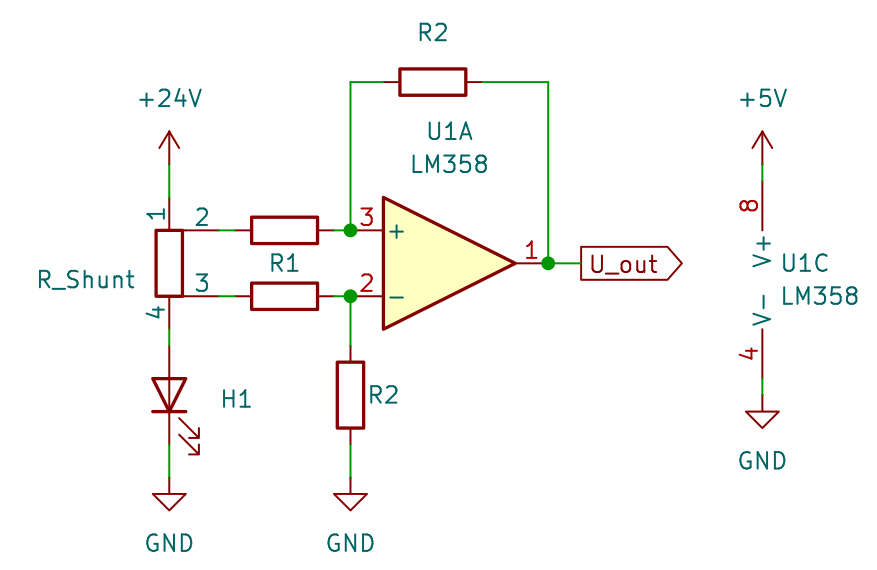
\includegraphics[width=1\textwidth]{images/sch.png}
		\caption{Schaltungsaufbau}
		\label{fig:HUB-Analyse}
	\end{figure}

\newpage

\subsection{Berechnungen:}
\begin{itemize}
\item $R_2=130k\Omega$ angenommen
\item $U_q = 24VDC$
\item $I_{ges}=844mA$ gemessen
\item $R_s = 15m\Omega$ Datenblatt \cite{RS}
\end{itemize}

\begin{align}
U_{RS} = Uq \cdot \frac{R_S}{\frac{U_q}{I_{ges}}}\\
U_a = \frac{R_2}{R_1}\cdot (U_q-U_{RS}-U_q)\\
5 = \frac{R_2}{R_1}\cdot 24.045V\\
R_1 = \frac{130k\Omega \cdot 24,045}{5} \approx 625\Omega
\end{align}


\subsection{Beobachtung:}
\begin{itemize}
    \item Die Schaltung hat nicht wie erwartet funktioniert.
    \item Der Differenzverstärker liefert keine korrekten Ausgangswerte.
\end{itemize}

\subsection{Ursachenanalyse:}
\begin{itemize}
    \item \textbf{GND-Problematik:} Wahrscheinlich liegt der Fehler an der Masseführung (GND). Bei High-Side-Messungen mit Differenzverstärkern kann es zu Problemen kommen, wenn Massepotenziale nicht richtig bezogen werden.
    \item \textbf{Potentialdifferenzen:} Bei High-Side-Konfigurationen besteht oft das Risiko von Offset-Fehlern oder falsch bezogenen Messpunkten aufgrund unsauberer Massebezüge.
\end{itemize}
\newpage

\subsection{Mögliche Lösung:}
\begin{itemize}
    \item \textbf{Massebezug überprüfen:} Sicherstellen, dass der Differenzverstärker korrekt geerdet ist und keine Masseverschiebungen auftreten.
    \item \textbf{Spannungspotenziale ausgleichen:} Eventuell eine galvanische Trennung oder eine präzisere Masseführung einbauen.
    \item \textbf{Alternative:} Low-Side-Messung in Betracht ziehen, da hier das GND-Problem einfacher zu handhaben ist.
    \item \textbf{Fertigen Differenzial OPV benutzen und nach typical Application von Datasheet benutzen:} \cite{INA}
    \begin{figure}[hbtp]
		\centering
		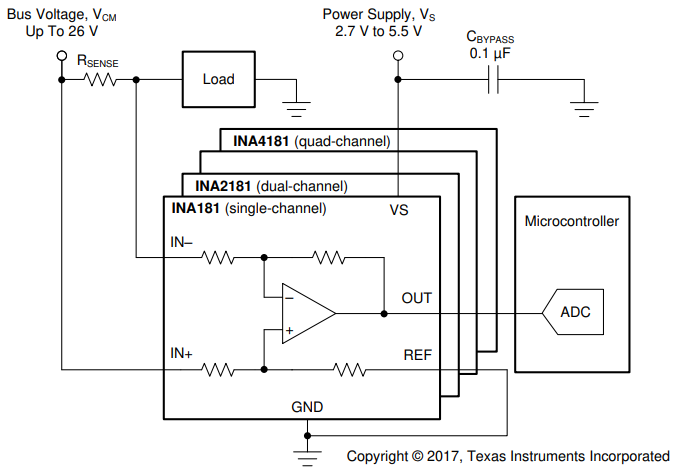
\includegraphics[width=1\textwidth]{images/new.png}
		\caption{Typical Application INA181}
		\label{fig:HUB-Analyse}
	\end{figure}
\end{itemize}

\subsection{Fazit:}
Die Fehlfunktion des Aufbaus lässt sich auf Probleme mit der Masseführung zurückführen, was bei High-Side-Messungen mit Differenzverstärkern häufig auftritt.




\newpage
\section{Literaturverzeichnis}
\begin{thebibliography}{9} % Die Zahl 9 ist die Breite für die Nummerierung
\bibitem{INA}
TEXAS INSTRUMENTS, 
\textit{INAx181 Bidirectional, Low- and High-Side Voltage Output,
Current-Sense Amplifiers Datasheet}, 
\url{https://www.ti.com/lit/ds/symlink/ina181.pdf}, 
Zugriff am 26.11.2024 um 02:55.

\bibitem{RS}
TEXAS INSTRUMENTS, 
\textit{Industry-Standard Dual Operational Amplifiers Datasheet}, 
\url{https://www.ti.com/lit/ds/symlink/lm358.pdf?ts=1732011604528&ref_url=https%253A%252F%252Fwww.ti.com%252Fproduct%252FLM358}, 
Zugriff am 26.11.2024 um 02:45.

\end{thebibliography}
\end{document}
